\section{Research Problem} \label{sec:Remark Problem}

SVC can help us to reduce network congestions but selecting some proper layer to stream isn't a optimal solution. The network condition would change violently in runtime. Select the packets in middle of Internet would be much better than decide them in the beginning. Nevertheless, regular switches in the Internet can't drop any particular packets. The working logic of them is such easy as store and forward all the packets. The packets will be drop without any remedy in UDP protocol which is the most used protocol in video streaming. In SVC sequence, the higher layer can be decode depends on the lower layer. In other words, forwarding the higher enhancement layer without the lower enhancement layer waste the network resource a lot. 

To solve this problem, we are going to use {\em Programming Protocol-Independent Packet Processors (P4)} ~\cite{BDGI+14} programming language to design a switch to drop some useless packets in the middle of the Internet. P4 is a new describing language with following features. (i) Protocol Independent, (ii) Target Independent, and (iii) Field Reconfigurable. Protocol independent allows us to design any protocol we want to forward the packet, and thus we can add some user-specific field in the header for us to make our decision. Target independent allows us to describe everything from high-performance ASICs to software switches. Field reconfigurable allows us to change the way our switches process packets after we deploy our p4 program. 

\begin{figure}[tbh]
    \centering
    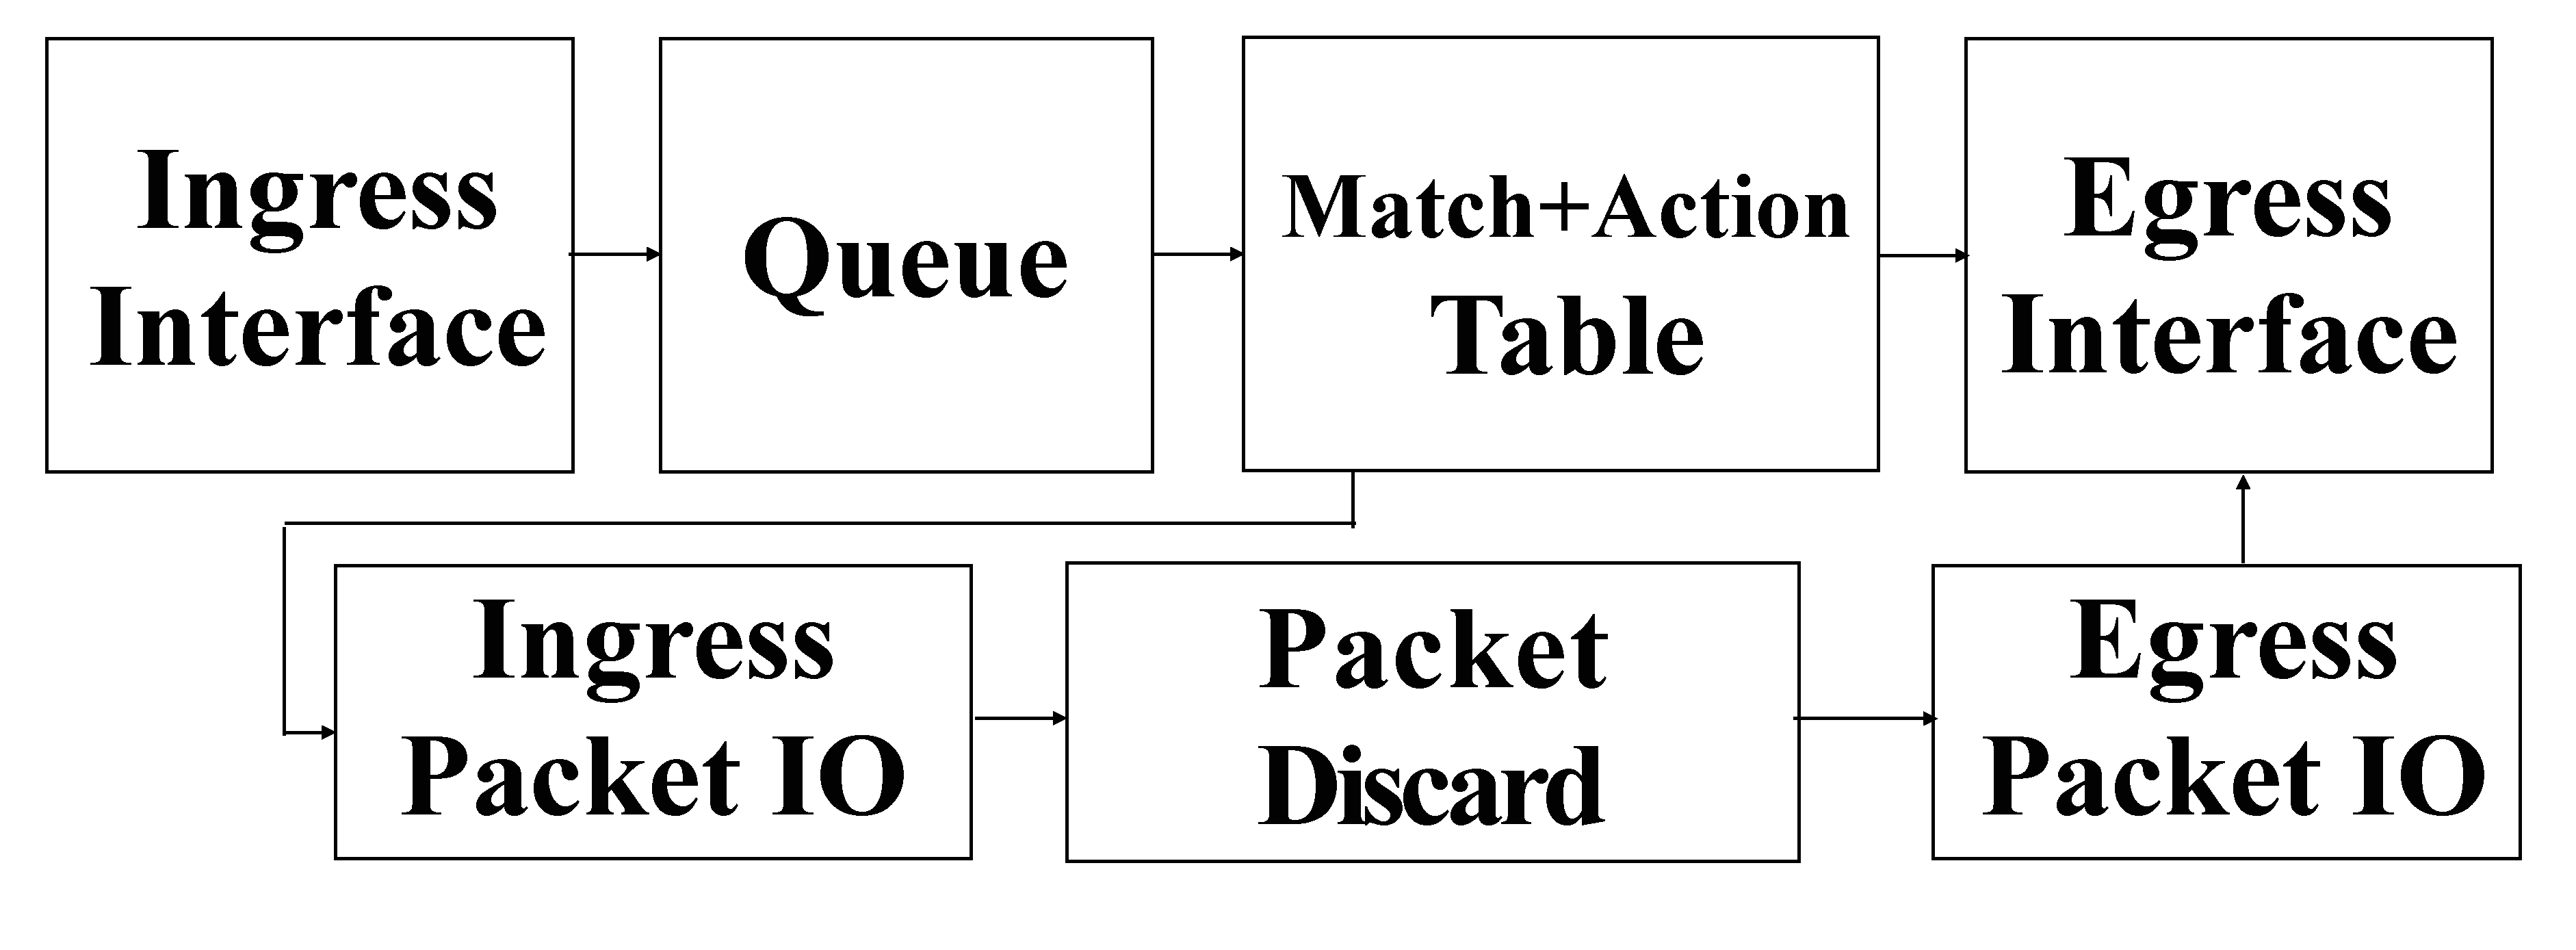
\includegraphics[width=.24\textwidth]{fig/MANE_1.eps}
    \caption{Packet processing in a P4-based MANE.}
    \label{MANE}
\end{figure}

Fig. ~\ref{MANE} shows how the P4-based MANE process packets. We define some header format and parsers which allow us to understand the structure of the packet. Incoming packets will first be parsed and divide into header and payload. We can design some match+action table in both ingress and egress control program to determine how to process the packet. In the ingress program, we can specify some match+action table to apply and may drop the packet if it's not valid or useless. After the packet pass the ingress program, it will be pushed into queues and than processed by the egress program. In P4, we can also calculate the checksum, configure forwarding table, construct some metadata adding to the header. With these tools and the knowledge of the whole Internet,  we can drop packets optimally in P4-based MANEs. 

On the other hand, P4-based MANE can not detect the condition of the whole Internet. Therefore, we combine P4-based MANE and SDN controller. Here we select {\em Open Network Operating System (ONOS)} to be our controller because it can from a controller plane without too many settings and it supports P4-runtime. P4-runtime is a program for controller to reconfig the P4-based MANEs. In other words, we can change the behavior of the P4-based MANE in runtime through P4-runtime. It works like a RESTful API server, we can simply give some commands to control our P4-based MANEs. 